\chapter{Inference-Time Scaling and Decoding}
\label{ch:inference-time-scaling}
\raggedbottom

In 2022, DeepMind's AlphaCode placed in the top 54\% of participants in competitive programming contests---roughly the level of a median human contestant~\cite{li2022competition}. Its method looked almost wasteful by ordinary chatbot standards. For each problem, the system sampled approximately one million candidate programs from a single fixed model, filtered them with example tests, clustered near-duplicates by runtime behavior, and submitted at most ten programs. No single sample was reliably correct. But across a million attempts, correct solutions almost always appeared, and a careful selection pipeline could find them. The striking lesson was not that brute-force sampling solved programming. It was that a fixed generator becomes a much stronger system when inference is treated as candidate generation plus selection.

Part~III ended with a trained assistant. It can follow instructions, answer preferences better than the base model, and sometimes solve math or code tasks by spending long reasoning traces. The next question is not yet multimodal, and it is not yet full agent design. The next question is simpler:

\begin{quote}
If the model weights are fixed, how much better can the system become by spending more computation at inference time?
\end{quote}

This is the entry point to Part~IV. A deployed model is not only a neural network. It is a runtime system: a prompt, a decoding rule, a sampling budget, a candidate-selection method, sometimes a verifier, sometimes a search procedure, and always a latency and cost budget. The same model can behave like a fast single-shot assistant or like a slower problem-solving system that samples, checks, votes, and searches.

One useful analogy is a writing room. Training improves the writer. Inference-time scaling keeps the writer fixed but asks for more drafts, gives those drafts to an editor, and sometimes asks for revisions before publishing one answer. More drafts help only if the writer can produce a useful alternative and the editor can recognize it. This analogy will thread through the chapter: decoding controls how each draft is written (Section~\ref{sec:ch18-decoding}), best-of-$N$ decides how many drafts to request (Section~\ref{sec:ch18-best-of-n}), self-consistency asks many drafters to vote (Section~\ref{sec:ch18-self-consistency}), verifiers play the editor (Section~\ref{sec:ch18-verifier-selection}), search lets the editor intervene mid-draft (Section~\ref{sec:ch18-search}), and the cost frontier asks how many drafts and edits the publishing budget can afford (Section~\ref{sec:ch18-cost-reliability}).

\paragraph{Chapter thesis.} \emph{Training sets the model's base distribution; inference-time methods decide how much computation we spend navigating, sampling, checking, and selecting from that distribution.} Inference-time scaling is not free capability. It converts compute into reliability only when useful candidates are present in the model's distribution and the runtime system can recognize them.

\paragraph{Running example.} Suppose your Project~3 assistant is asked a contest-style algebra problem. A greedy answer is often wrong. If you sample 32 independent solutions, several may be correct. If you can identify the correct one with an answer checker, majority vote, or process verifier, the system becomes much more reliable without changing weights. If all 32 samples make the same conceptual mistake, more sampling only makes the failure more expensive. This chapter is about that boundary.

\subsection*{Learning Objectives}

After completing this chapter, you should be able to:

\begin{enumerate}
  \item Explain why autoregressive models define token distributions rather than direct answers.
  \item Compare greedy decoding, temperature sampling, top-$k$, top-$p$, and beam search.
  \item Compute simple pass@$k$ and best-of-$N$ reliability estimates.
  \item Explain when self-consistency helps reasoning and when correlated failures defeat it.
  \item Describe verifier-guided selection as a runtime system rather than a training objective.
  \item Distinguish model-internal reasoning search from tool-using agent loops.
  \item Analyze the cost--latency--reliability trade-off of inference-time scaling.
\end{enumerate}

\subsection*{Notation}

\begin{center}
\begin{tabularx}{\textwidth}{@{}lX@{}}
\toprule
Symbol & Meaning \\
\midrule
$p_\theta(x_t \mid x_{<t})$ & Next-token distribution produced by an autoregressive model \\
$T$ & Sampling temperature; lower $T$ sharpens the distribution, higher $T$ flattens it \\
$N$ or $k$ & Number of sampled candidates or attempts \\
$p$ & Single-attempt success probability when a task has a binary success criterion \\
$q$ & Probability that a selector or verifier chooses a correct candidate when one exists \\
$C_{\text{gen}}, C_{\text{score}}$ & Approximate cost of generating one candidate and scoring one candidate \\
\bottomrule
\end{tabularx}
\end{center}

\subsection*{Timeline of Key Contributions}

\begin{center}
\begin{tabularx}{\textwidth}{@{}lX@{}}
\toprule
\textbf{Year} & \textbf{Milestone} \\
\midrule
2020 & GPT-3 popularizes few-shot prompting and sample-based evaluation for large autoregressive models~\cite{brown2020language}. \\
2020 & Nucleus sampling argues that truncating the unreliable probability tail improves open-ended generation~\cite{holtzman2020curious}. \\
2021 & GSM8K pairs math word problems with verifier-style reasoning evaluation~\cite{cobbe2021gsm8k}. \\
2023 & Self-consistency shows that sampling multiple chain-of-thought solutions and voting improves reasoning accuracy~\cite{wang2022selfconsistency}. \\
2023 & Step-by-step verification studies process reward models for selecting and supervising reasoning traces~\cite{lightman2023verify}. \\
2023 & Tree-of-Thoughts frames test-time reasoning as search over intermediate thoughts rather than one left-to-right sample~\cite{yao2023tree}. \\
2024 & Test-time compute scaling becomes an explicit scaling-law question: when should we spend more compute during inference instead of training a larger model?~\cite{snell2024scaling}. \\
2024--2025 & o1 and DeepSeek-R1 make deliberate inference-time computation a central public feature of reasoning models~\cite{openai2024reasoning,deepseekai2025r1}. \\
\bottomrule
\end{tabularx}
\end{center}

\paragraph{What this chapter covers.} The chapter begins with decoding because sampling is the source of candidate diversity. It then moves from single samples to candidate pools, from candidate pools to voting and verifier-guided selection, and from flat reranking to model-internal search over reasoning traces. The chapter ends by putting all of these methods on a cost--latency--reliability frontier. The goal is not to memorize every decoding trick. The goal is to see inference as a controllable runtime algorithm around a fixed model.


%----------------------------------------------------------------------
\section{Why Inference-Time Scaling Matters}
\label{sec:ch18-why}

The first three parts of this book mostly studied how model weights are produced: architecture, data, pretraining, SFT, preference optimization, and reasoning RL. Inference-time scaling studies a different axis. Once the weights are fixed, a system designer still chooses how many tokens to generate, how many candidates to sample, whether to score them, whether to vote, whether to search over partial reasoning paths, and when to stop.

This is not a minor implementation detail. The user sees a system, not a raw conditional distribution. A model with weak pass@1 but strong pass@64 can be useless in a low-latency chat setting and valuable in a batch problem-solving setting. A model with strong single-sample accuracy may not benefit much from extra sampling. A slow verifier may improve accuracy but make the product unusable. The system's quality is therefore a function of both model capability and runtime allocation.

\paragraph{The bridge from Ch17.} Chapter~\ref{ch:frontiers} used pass@$k$ as an epistemic diagnostic: if the base model catches up at large $k$, perhaps RL surfaced behavior rather than created it. This chapter uses the same idea operationally. If correct answers exist somewhere in the model's sample distribution, inference-time compute is the mechanism for finding them.

\paragraph{Training compute versus inference compute.} Part~II introduced training scaling: parameters, data, and training compute. In deployment, total compute includes inference. A smaller model sampled many times can sometimes outperform a larger model sampled once on tasks where candidate diversity and selection are strong. Snell et al.\ make this explicit: test-time compute can be allocated across sampling, revision, and verification, and the best allocation depends on task difficulty, model size, and the quality of the selection procedure~\cite{snell2024scaling}. This does not overturn training scaling laws. It adds another frontier: \emph{compute-optimal inference}.

\paragraph{Reasoning models blur the boundary.} o1 and DeepSeek-R1 make this topic especially timely~\cite{openai2024reasoning,deepseekai2025r1}. These models were trained with RL to produce long chains of thought (Chapter~\ref{ch:reasoning-rl}), and they also spend substantially more tokens per answer at inference time. Their improved performance comes from \emph{both} training-time and inference-time compute. This chapter isolates the inference side: for a model with fixed weights, what does the runtime procedure add? Reasoning models are one answer---they use fixed weights that were trained to be amenable to long inference-time search---but the inference-time scaling idea is more general than any single model family.

\paragraph{What changes at runtime.} Inference-time methods can change three things without changing weights:

\begin{enumerate}[nosep]
  \item \textbf{Which candidate is sampled}: decoding controls diversity, determinism, and tail risk.
  \item \textbf{How many candidates are considered}: best-of-$N$ and self-consistency turn one attempt into a small population.
  \item \textbf{How candidates are selected or expanded}: verifiers, reward models, voting, and search decide where extra compute goes.
\end{enumerate}

The rest of the chapter follows that progression: decoding, candidates, selection, ensembles, verification, search, and finally the cost--reliability frontier.

\begin{figure}[t]
\centering
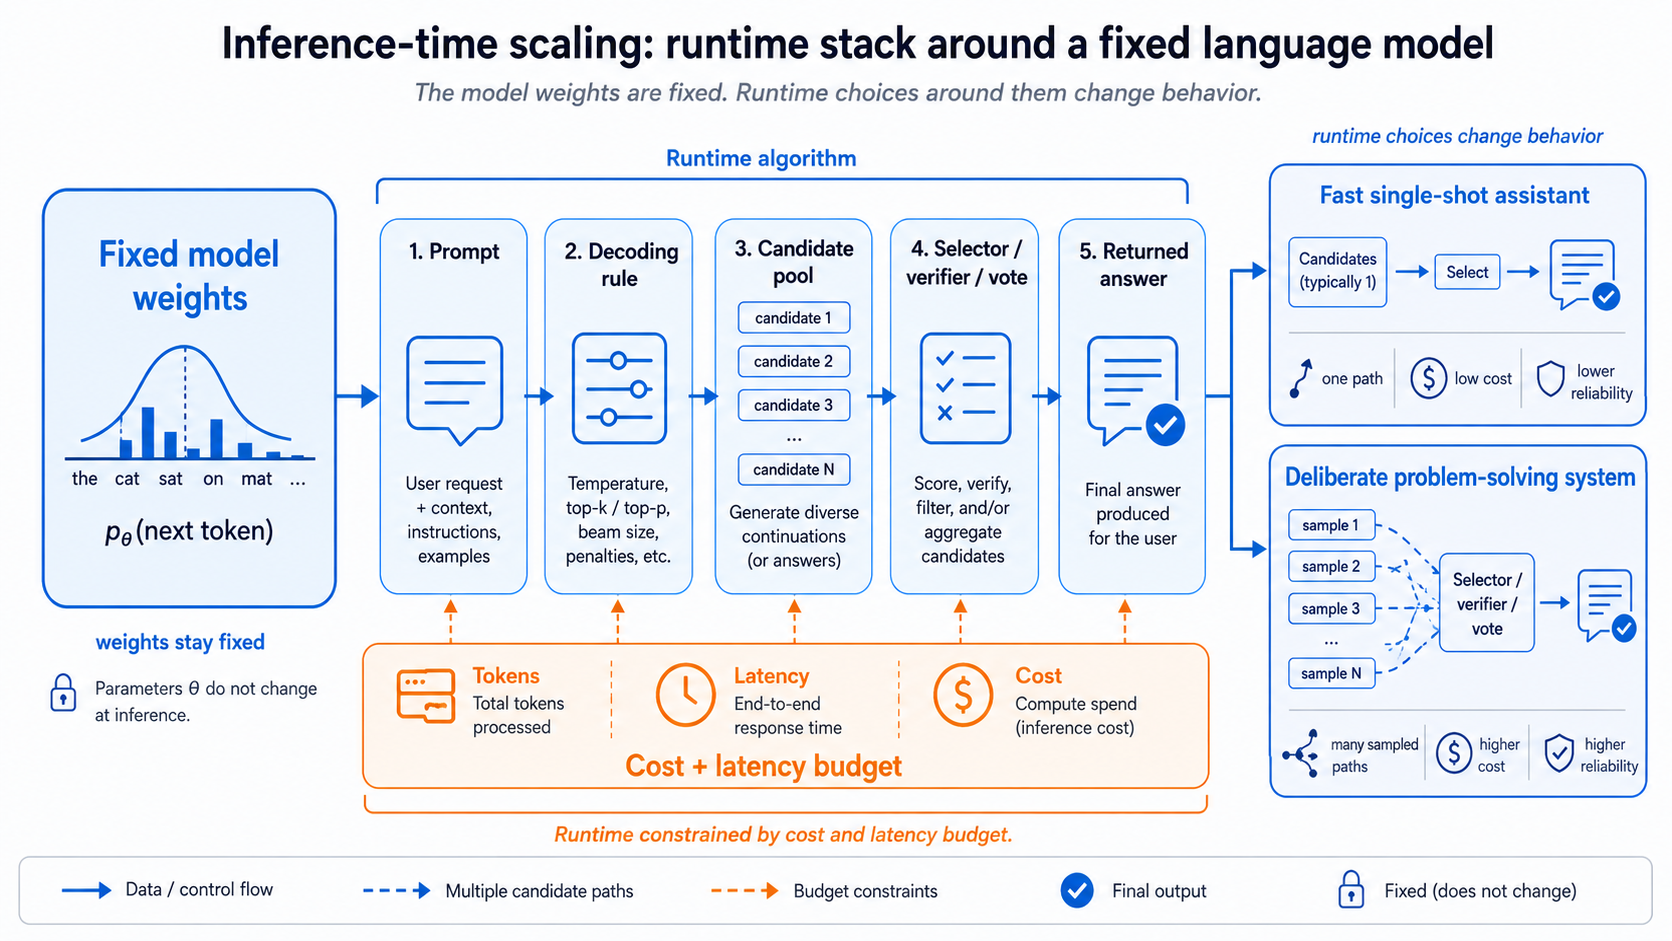
\includegraphics[width=0.95\textwidth]{figures/ch18/fig_runtime_compute_stack.png}
\caption{Inference-time scaling as a runtime stack. A fixed model distribution is wrapped by decoding, candidate generation, selection, search, and a cost budget. The system's behavior is the whole stack, not the weights alone.}
\label{fig:ch18-runtime-compute-stack}
\end{figure}

\begin{tcolorbox}[colback=blue!5, colframe=blue!40, title=\textbf{Is Inference-Time Scaling Real Capability?}]
There are two defensible answers. From the user's perspective, a system that solves more tasks with the same weights is more capable. From the model-audit perspective of Chapter~\ref{ch:frontiers}, extra samples may only reveal behavior already present in the model's distribution. Ch18 uses the systems answer: runtime compute is real capability for the deployed system, even when it is not evidence that the model's weights learned a new internal algorithm.
\end{tcolorbox}

\begin{quickrecap}
\textbf{Quick Recap.}
\begin{itemize}[nosep,leftmargin=1.5em]
  \item Inference-time scaling improves a fixed model by spending more runtime compute.
  \item It is the operational counterpart to Ch17's pass@$k$ diagnostic.
  \item The key question is not ``does more compute help?'' but ``where should the compute be spent?''
\end{itemize}
\textit{Next: the model gives a token distribution, so decoding decides how a candidate is born.}
\end{quickrecap}


%----------------------------------------------------------------------
\section{Decoding as Distribution Navigation}
\label{sec:ch18-decoding}

An autoregressive language model does not directly output an answer. At each step it produces a distribution over the next token:

\begin{equation}
  p_\theta(x_t \mid x_{<t}).
  \label{eq:next-token-distribution}
\end{equation}

Generation is the process of repeatedly turning this distribution into a token, appending that token to the context, and asking for the next distribution. A decoding strategy is therefore a policy for navigating the model's token distribution. Project~1 used temperature and top-$k$ sampling as an implementation exercise. Here we need the conceptual version, because every inference-scaling method depends on what kind of candidates decoding produces.

\subsection{Greedy Decoding}

Greedy decoding chooses the most likely token at every step:

\begin{equation}
  x_t = \arg\max_x p_\theta(x \mid x_{<t}).
\end{equation}

This is fast, deterministic, and often good for short factual completions. It is also brittle. Locally likely tokens do not always lead to the best global answer. In reasoning tasks, the first plausible step can commit the model to a bad path. In creative tasks, greedy decoding often becomes repetitive or bland because it repeatedly chooses high-probability continuations.

In the running algebra example, greedy decoding is the ``first solution on the whiteboard.'' It may be correct, but if it makes an early algebraic substitution error, every later token is conditioned on that mistake. Greedy decoding is useful as a baseline because it asks: what does the model do when we spend almost no search compute? But it should not be confused with the model's full capability. It reads one path through a distribution, not the distribution itself.

\subsection{Temperature Sampling}

Temperature rescales logits before the softmax:

\begin{equation}
  p_T(x \mid x_{<t}) =
  \frac{\exp(z_x/T)}{\sum_{x'} \exp(z_{x'}/T)}.
  \label{eq:temperature}
\end{equation}

When $T<1$, the distribution becomes sharper: high-probability tokens become even more likely. When $T>1$, the distribution becomes flatter: lower-probability tokens are sampled more often. At $T \to 0$, temperature sampling approaches greedy decoding.

The practical trade-off is simple. Low temperature improves determinism and reduces incoherent tails, but it may suppress useful alternative solution paths. High temperature increases diversity, but it spends samples on noise. Reasoning pipelines often use moderate temperatures because best-of-$N$ and self-consistency require candidate diversity; if all candidates are nearly identical, sampling $N$ times is expensive determinism.

\subsection[Top-k and Top-p Sampling]{Top-$k$ and Top-$p$ Sampling}

The raw distribution has a long tail. Many tokens have tiny probability but are not impossible. Sampling from that full tail can produce incoherent or unsafe continuations. Two common truncation methods remove much of that tail.

\paragraph{Top-$k$.} Keep only the $k$ most likely tokens, renormalize their probabilities, and sample from that truncated set. Small $k$ is conservative; large $k$ allows more diversity.

\paragraph{Top-$p$ or nucleus sampling.} Sort tokens by probability and keep the smallest set whose cumulative probability is at least $p$. This adapts the candidate set size to uncertainty. If the model is confident, the nucleus may contain only a few tokens. If the model is uncertain, the nucleus may be larger. Holtzman et al.\ argued that nucleus sampling helps avoid the unreliable tail while preserving open-ended diversity~\cite{holtzman2020curious}.

For reasoning, truncation is not only about prose quality. It shapes the candidate pool. Too much truncation makes best-of-$N$ redundant; too little makes it noisy. The right decoding setting depends on the downstream selector. If a strong verifier can reject bad candidates cheaply, a higher-diversity pool may be useful. If there is no selector, conservative decoding is safer.

\subsection{Beam Search}

Beam search keeps the top $B$ partial sequences under the model likelihood and expands them step by step. It is a classic decoding method in machine translation, where high-likelihood sequences often correlate with quality. For open-ended LLM generation, beam search is less dominant. High model likelihood can favor generic, repetitive, or overly safe text. For reasoning, beam search over token likelihood is also misaligned: the most likely proof-looking sequence is not necessarily the correct solution.

This does not make beam search irrelevant. It teaches an important lesson: search needs the right scoring function. Searching over token likelihood alone is not the same as searching over task success. The rest of this chapter replaces pure likelihood with selection signals that better match the task: answer agreement, verifiers, process scores, and structured reasoning search.

\begin{figure}[t]
\centering
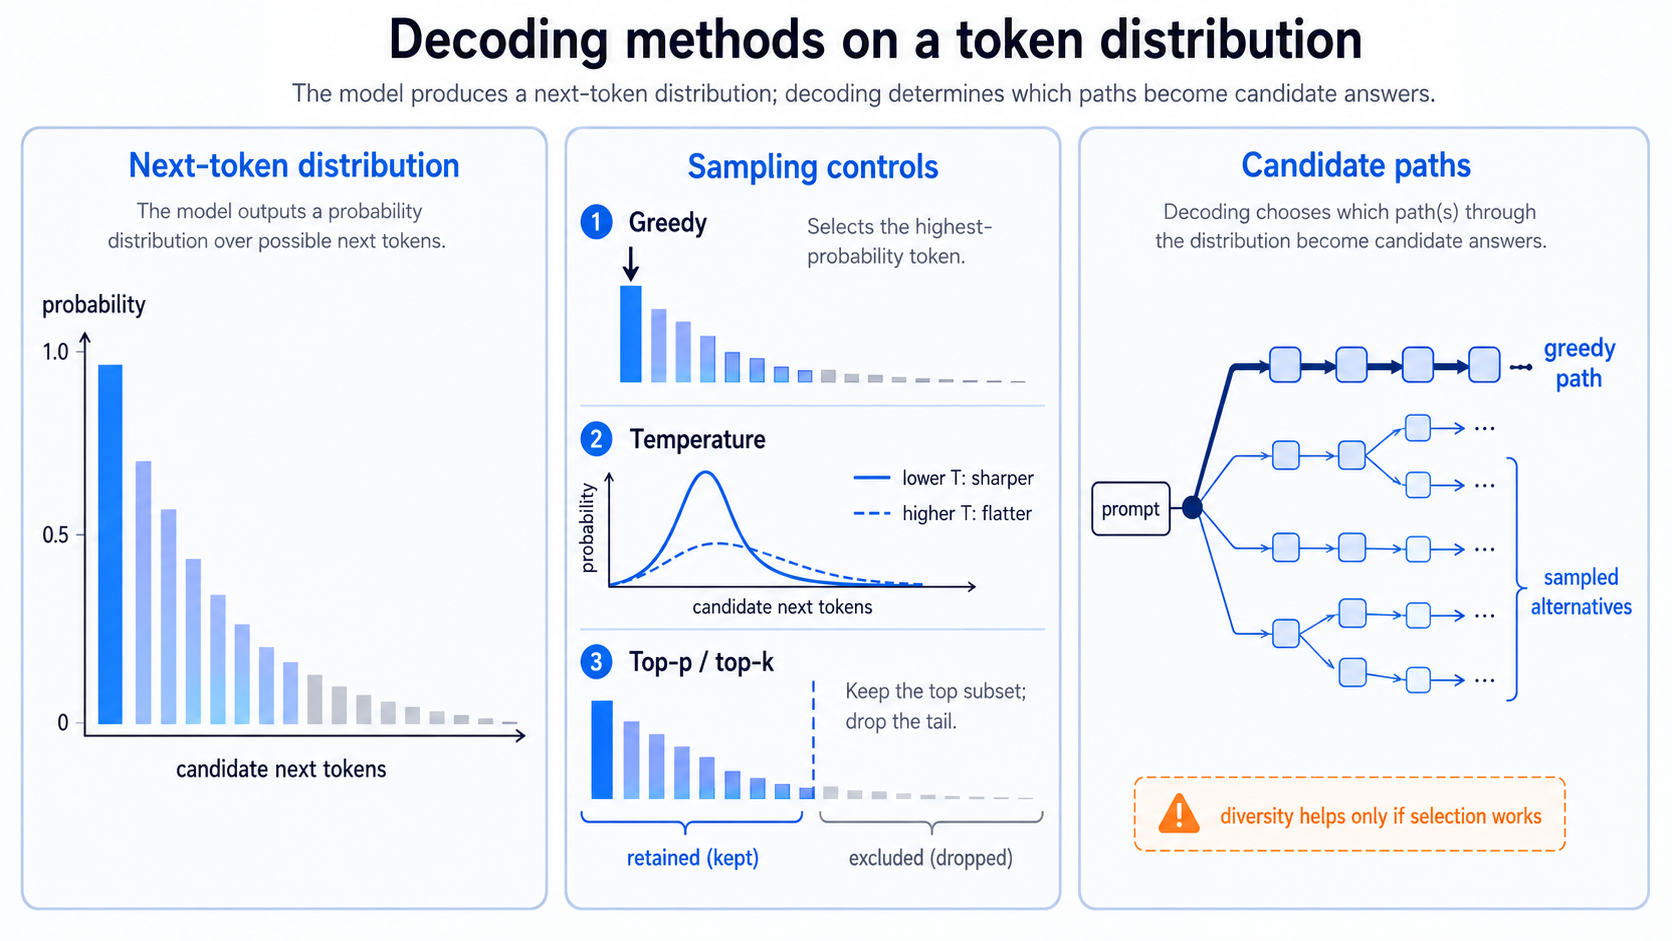
\includegraphics[width=0.95\textwidth]{figures/ch18/fig_decoding_distribution.png}
\caption{Decoding as distribution navigation. Greedy decoding follows the highest-probability token path; temperature and truncation methods expose alternative paths; beam search keeps high-likelihood prefixes. Candidate diversity begins at the decoding layer.}
\label{fig:ch18-decoding-distribution}
\end{figure}

\begin{center}
\small
\begin{tabularx}{\textwidth}{@{}p{2.8cm}p{3.2cm}p{3.5cm}X@{}}
\toprule
\textbf{Method} & \textbf{Main control} & \textbf{Strength} & \textbf{Failure mode} \\
\midrule
Greedy & Always choose max-prob token & Fast, deterministic baseline & One brittle path; no diversity \\
Temperature & Sharpen or flatten logits & Controls diversity smoothly & Too low collapses; too high adds noise \\
Top-$k$ & Fixed candidate set size & Removes extreme tail & Same $k$ may be too wide or narrow by context \\
Top-$p$ & Cumulative probability mass & Adaptive tail truncation & Sensitive to $p$ and model calibration \\
Beam search & Keep high-likelihood prefixes & Structured likelihood search & Likelihood can disagree with task success \\
\bottomrule
\end{tabularx}
\normalsize
\end{center}

\begin{quickrecap}
\textbf{Quick Recap.}
\begin{itemize}[nosep,leftmargin=1.5em]
  \item Decoding turns a next-token distribution into a candidate sequence.
  \item Diversity is not automatically good; it is useful only if the system can select from it.
  \item Beam search shows why likelihood search and task-success search are different.
\end{itemize}
\textit{Next: once decoding can produce multiple candidates, inference-time scaling becomes a selection problem.}
\end{quickrecap}


%----------------------------------------------------------------------
\section{Best-of-N, Pass@k, and Candidate Selection}
\label{sec:ch18-best-of-n}

The simplest inference-scaling method is to sample multiple candidates and keep the best one. The difficult word is \emph{best}. If the task has an exact verifier, best can mean correct. If the task has a reward model, best can mean highest reward. If the task has no reliable judge, best-of-$N$ may only select the most plausible-looking answer.

\subsection{Pass@k as Runtime Opportunity}

Suppose one sampled answer succeeds with probability $p$, and suppose samples are independent. The probability that at least one of $k$ samples succeeds is:

\begin{equation}
  \Pr(\text{at least one success}) = 1 - (1-p)^k.
  \label{eq:passk-runtime}
\end{equation}

This equation is optimistic because real samples are correlated. Still, it gives the first-order intuition. A model with $p=0.20$ has only 20\% single-shot success, but eight independent attempts contain at least one success with probability:

\begin{equation}
  1 - 0.8^8 \approx 0.832.
\end{equation}

That does not mean the final system is 83.2\% accurate. It means the candidate pool contains a correct answer that often. The system still needs to identify it.

For the running algebra problem, this is the difference between ``the model solved it once'' and ``one of the 32 scratch-work attempts contains the right derivation.'' best-of-$N$ is useful only if the runtime system can find that derivation instead of returning a fluent but wrong one.

\noindent\fbox{\parbox{\dimexpr\textwidth-2\fboxsep-2\fboxrule\relax}{%
\textbf{Pause and verify.}\quad A model has independent single-sample success probability $p=0.2$. (a) What is the probability that at least one of $8$ samples is correct? (b) If a selector chooses a correct candidate with probability $q=0.7$ whenever at least one exists, what is the final system accuracy? (c) How does your answer change if the samples are highly correlated and the effective number of independent attempts is only $4$?
}}

\subsection{Selection Quality}

Best-of-$N$ has two stages: generate candidates, then select. The generation stage asks whether a correct answer appears. The selection stage asks whether the system recognizes it. A rough decomposition is:

\begin{equation}
  \Pr(\text{system success}) \approx
  \Pr(\text{at least one correct candidate}) \cdot
  \Pr(\text{selector chooses correct} \mid \text{one exists}).
  \label{eq:selection-decomposition}
\end{equation}

This is why selection quality can bottleneck inference-time scaling. If the selector is random among $N$ candidates, more samples may make selection harder. If the selector is a perfect verifier, more samples help until candidate generation saturates. If the selector is a learned reward model with blind spots, best-of-$N$ can amplify those blind spots. This is the runtime version of reward overoptimization from Chapter~\ref{ch:rlhf}: selecting the maximum over many candidates increases pressure on the score.

\begin{figure}[t]
\centering
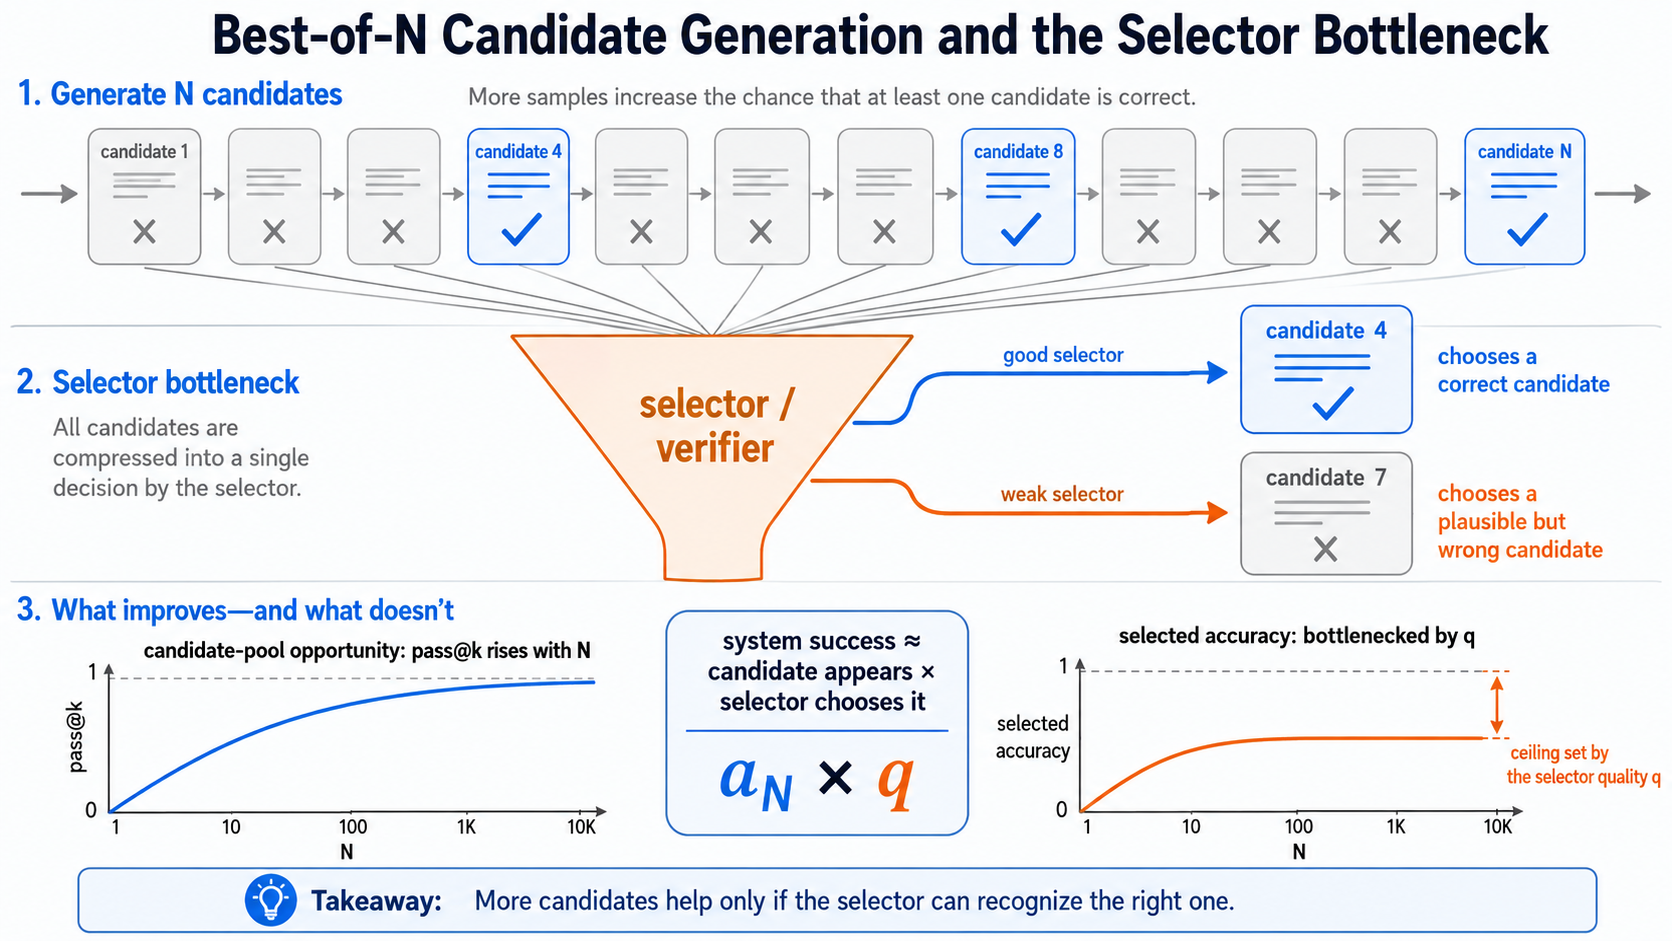
\includegraphics[width=0.95\textwidth]{figures/ch18/fig_bestofn_selection_bottleneck.png}
\caption{Best-of-$N$ separates candidate availability from selector quality. More samples can make a correct answer appear, but final accuracy depends on whether the selector can identify it.}
\label{fig:ch18-bestofn-selection-bottleneck}
\end{figure}

\subsection{Diversity, Correlation, and Diminishing Returns}

Equation~\ref{eq:passk-runtime} assumes independence. LLM samples are not independent in the way coin flips are independent. They are drawn from the same model, prompted in the same way, and often share the same dominant misconception. Increasing $N$ then yields diminishing returns: the tenth sample may be much less informative than the first.

There are three practical ways to improve the candidate pool:

\begin{enumerate}[nosep]
  \item \textbf{Sampling diversity}: tune temperature, top-$p$, and prompt variants to avoid identical trajectories.
  \item \textbf{Problem decomposition}: ask for different solution approaches rather than many copies of the same approach.
  \item \textbf{Adaptive stopping}: stop early when candidates agree under a reliable check, and spend more compute when disagreement remains.
\end{enumerate}

The system question is not ``what is the largest $N$ we can afford?'' It is ``which additional sample is likely to change the decision?''

\begin{quickrecap}
\textbf{Quick Recap.}
\begin{itemize}[nosep,leftmargin=1.5em]
  \item pass@$k$ measures whether a candidate pool contains a success.
  \item best-of-$N$ also needs a selector; weak selectors can waste or invert the benefit of more samples.
  \item Correlated samples make naive independence calculations overestimate gains.
\end{itemize}
\textit{Next: self-consistency uses multiple reasoning traces when exact selection is unavailable.}
\end{quickrecap}


%----------------------------------------------------------------------
\section{Self-Consistency and Reasoning Ensembles}
\label{sec:ch18-self-consistency}

Chain-of-thought prompting made reasoning traces visible. Self-consistency made those traces into an inference-time ensemble. Instead of taking the first chain of thought, sample multiple reasoning paths, extract their final answers, and choose the answer that appears most often~\cite{wang2022selfconsistency}.

The method is simple:

\begin{enumerate}[nosep]
  \item Prompt the model to solve with reasoning.
  \item Sample $N$ reasoning traces at a nonzero temperature.
  \item Extract the final answer from each trace.
  \item Aggregate by majority vote, plurality vote, or answer clustering.
\end{enumerate}

Self-consistency works when different reasoning paths make partially independent errors. If five traces reach answer A and one trace reaches answer B, A is not guaranteed correct, but agreement is evidence. In the writing-room analogy, self-consistency hires several writers independently and asks them to vote on the answer, with no editor in the loop. The method is especially useful when exact verification is unavailable but answers have a stable form.

In the algebra example, self-consistency might sample one solution by substitution, another by factoring, and another by simplifying both sides before solving. If three independent-looking traces converge on the same value of $x$, agreement is informative. If all traces copy the same invalid cancellation step, agreement is only shared error.

\paragraph{Why it helps.} A single chain of thought can fail because of an arithmetic slip, a bad decomposition, or an early commitment. Sampling several traces gives the model several chances to route around those local failures. Majority vote then acts like an error-correcting layer if correct reasoning paths are more likely to agree than incorrect ones.

\paragraph{When it fails.} Self-consistency fails when errors are correlated. If the model has a strong but wrong prior, all traces may repeat the same misconception. It also fails when final-answer extraction is ambiguous, when multiple valid answers exist, or when the majority answer is merely the most common shortcut. In these cases, agreement measures confidence, not correctness.

\paragraph{Reasoning traces as search objects.} The important shift is that reasoning is no longer only explanatory text. It becomes a runtime object that can be sampled, compared, voted on, and scored. Chapter~\ref{ch:reasoning-rl} showed that reasoning traces can be reinforced during training. This chapter shows that they can also be ensembled at inference time.

\begin{figure}[t]
\centering
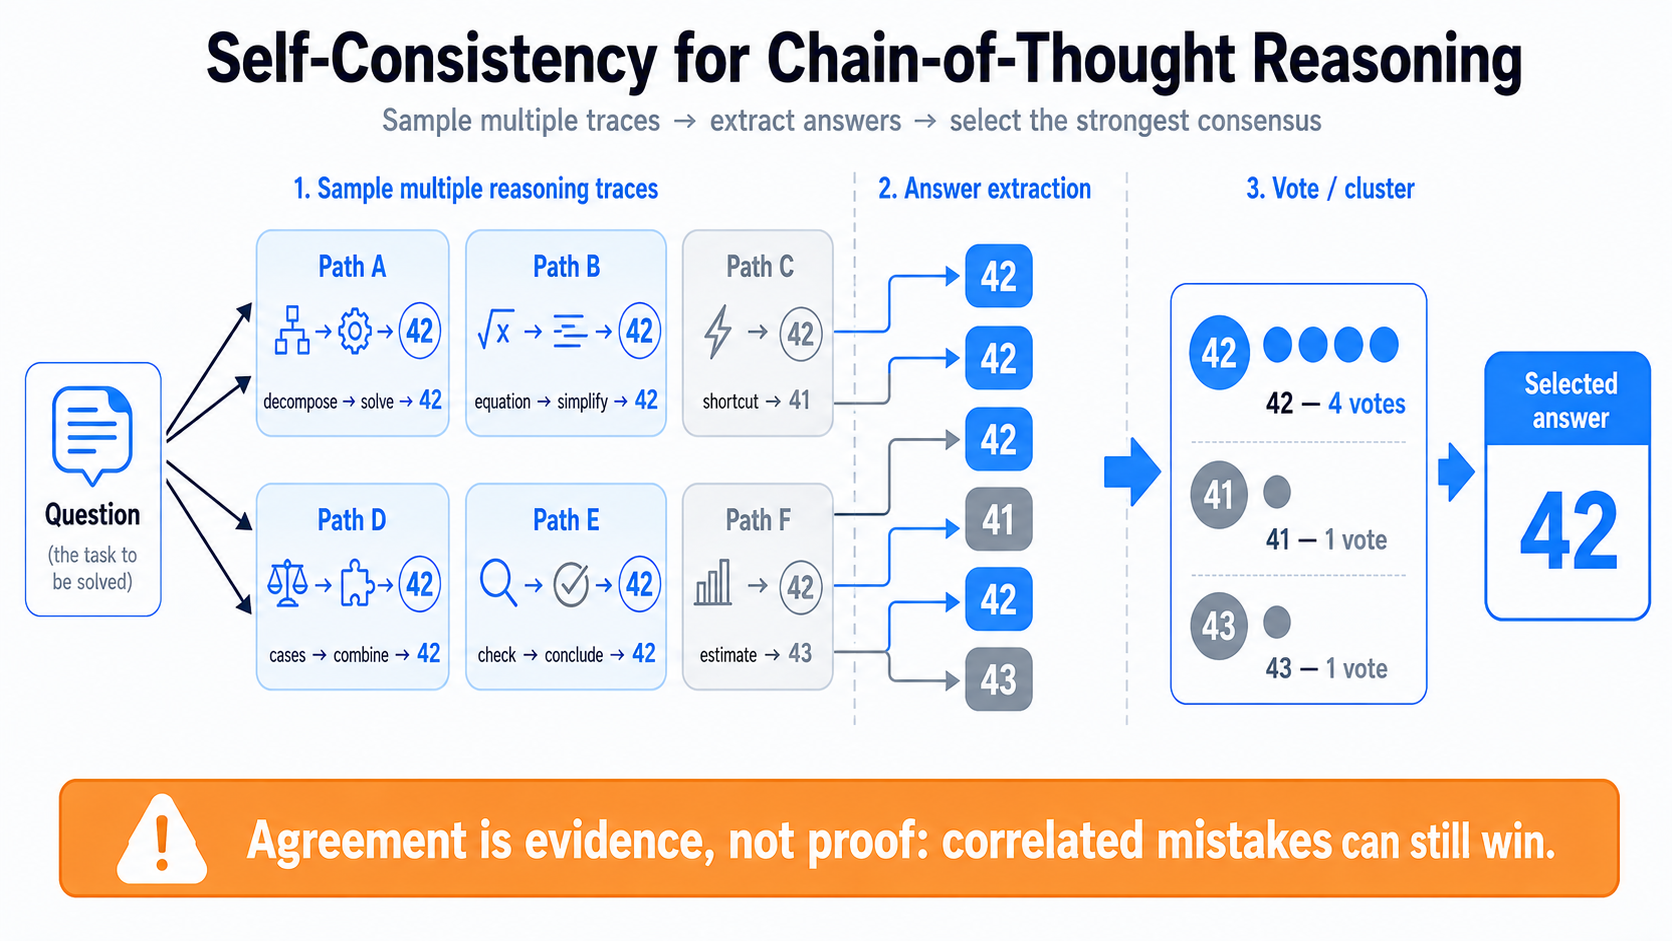
\includegraphics[width=0.95\textwidth]{figures/ch18/fig_self_consistency_pipeline.png}
\caption{Self-consistency turns one prompt into a small reasoning ensemble. Multiple sampled traces produce final answers; aggregation uses answer agreement as a weak selection signal.}
\label{fig:ch18-self-consistency-pipeline}
\end{figure}

\begin{center}
\small
\begin{tabularx}{\textwidth}{@{}p{3cm}p{4.5cm}X@{}}
\toprule
\textbf{Setting} & \textbf{Why self-consistency helps} & \textbf{Main risk} \\
\midrule
Math word problems & Different decompositions can cancel arithmetic or planning slips & Shared wrong setup dominates all traces \\
Symbolic reasoning & Final answers are easy to cluster or compare & Model may converge on common invalid shortcut \\
Open-ended advice & Multiple perspectives reveal uncertainty & Voting has no clear correctness target \\
Code design & Several implementations expose alternatives & Final-answer vote is meaningless without execution \\
\bottomrule
\end{tabularx}
\normalsize
\end{center}

\begin{quickrecap}
\textbf{Quick Recap.}
\begin{itemize}[nosep,leftmargin=1.5em]
  \item Self-consistency turns multiple chain-of-thought samples into a reasoning ensemble.
  \item It helps when errors are partially independent and final answers can be aggregated.
  \item It fails when samples share the same misconception or when there is no stable answer to vote on.
\end{itemize}
\textit{Next: instead of voting, a system can score candidates with a verifier.}
\end{quickrecap}


%----------------------------------------------------------------------
\section{Verifier-Guided Selection and Scaling}
\label{sec:ch18-verifier-selection}

Chapter~\ref{ch:reasoning-rl} introduced verifiable rewards for training. Chapter~\ref{ch:frontiers} audited what those rewards reveal or hide. Here we use verifiers differently: as runtime selection mechanisms.

A verifier-guided inference pipeline has a simple shape:

\begin{enumerate}[nosep]
  \item Generate $N$ candidate responses.
  \item Score each response with a verifier, reward model, unit test, answer checker, or process model.
  \item Return the highest-scoring response, or use the scores to guide more search.
\end{enumerate}

The key question is not what a verifier is; previous chapters already covered that. The key question is how verifier quality changes the scaling curve.

\subsection{Outcome Selection}

An outcome verifier scores a completed answer. Math answer checking and unit tests are the cleanest examples. In these settings, best-of-$N$ can be powerful because selection is close to exact: if any candidate passes, return it. Cobbe et al.\ used trained verifiers for math word problems, and modern code systems use execution feedback in the same spirit~\cite{cobbe2021gsm8k}.

Outcome selection is cheap when the verifier is a script. It is expensive when the verifier is a large model. It is brittle when the checker covers only part of the real task. A code solution that passes visible tests may fail hidden edge cases. A math solution with a correct final answer may contain invalid reasoning. Runtime verification improves the system only for the properties it checks.

For the algebra problem, an outcome checker can substitute the proposed $x$ back into the original equation. That is powerful because it checks the target directly. It still does not certify that the written reasoning was valid; it certifies that the final value satisfies the equation under the checker.

\subsection{Process Selection}

A process verifier scores intermediate reasoning steps. Lightman et al.\ showed that step-level supervision can be more informative for mathematical reasoning than only judging final answers~\cite{lightman2023verify}. At inference time, a process verifier can rank partial traces, prune bad branches, or prefer candidates with locally valid steps.

Process selection changes the scaling behavior because it can spend compute before a full answer is generated. Instead of sampling 64 complete solutions and scoring them at the end, the system can expand promising partial paths and abandon weak ones. This is closer to search than reranking.

\subsection{The Selector Bottleneck}

Suppose the candidate pool contains a correct answer with probability $a_N$, and the selector chooses a correct candidate with probability $q$ when one exists. Then final accuracy is roughly $a_N q$. Increasing $N$ improves $a_N$ but may reduce $q$ if the candidate pool becomes harder to judge or contains more reward-model adversarial examples.

This creates three regimes:

\begin{description}[leftmargin=1.5em]
  \item[Generator-limited.] Correct candidates rarely appear. Spend compute on better prompts, higher-quality base models, or training; selection cannot choose what is absent.
  \item[Selector-limited.] Correct candidates appear, but the verifier often misses them. Spend compute on better selection, process checks, or independent judges.
  \item[Cost-limited.] Correct candidates and selection both work, but latency or budget prevents large $N$. Spend compute adaptively.
\end{description}

Inference-time scaling is strongest in the middle: the model can sample useful candidates, and the selector is reliable enough to identify them.

\paragraph{A concrete example.} Suppose each sample solves the algebra problem independently with probability $p = 0.25$. With $N=16$ samples, the candidate pool contains at least one correct solution with probability $a_{16} = 1 - 0.75^{16} \approx 0.99$. If an outcome verifier identifies the correct solution with probability $q = 0.8$, the system's accuracy is roughly $0.99 \times 0.8 = 0.79$. Now consider a process verifier with $q = 0.95$: the system jumps to $0.94$. Or consider a weaker model with $p = 0.05$: even at $N = 16$, $a_{16} = 1 - 0.95^{16} \approx 0.56$, and with $q = 0.8$ the system only reaches $0.45$. The bottleneck has shifted from selector to generator. These numbers are stylized, but the diagnostic question is real: is your system failing because correct candidates are absent, or because the selector cannot find them?

\begin{tcolorbox}[colback=blue!5, colframe=blue!40, title=\textbf{Is Process Verification Always Better Than Outcome Verification?}]
Not necessarily. Process verifiers require step-level labels or a model that can judge intermediate reasoning, which is harder to build and harder to validate than a final-answer checker. If the outcome verifier is near-exact---a unit test, an equation substitution, a formal proof checker---it may be both cheaper and more reliable than a learned process model. Process verification is most valuable when: (1) generating a complete answer is expensive, so pruning early saves substantial compute; (2) outcome verification is unreliable or incomplete, as when tests cover only part of the specification; or (3) the system needs to explain \emph{why} an answer is correct, not just \emph{that} it is correct. In the writing-room analogy, outcome verification is publishing only the stories that sell. Process verification is an editor who reads drafts paragraph by paragraph and says ``this plot thread will not resolve---cut it now.''
\end{tcolorbox}

\begin{tcolorbox}[colback=gray!8, colframe=gray!40, title=\textbf{Echo: From Ch17 Audit to Ch18 Runtime}]
Chapter~\ref{ch:frontiers} asked whether pass@$k$ evidence means RL created new capability or merely concentrated probability on existing successful trajectories. Ch18 turns the same distinction into an engineering recipe. If the solution is already in the sample distribution, runtime selection can expose it. If it is outside the distribution, no amount of reranking can select it.
\end{tcolorbox}

\begin{quickrecap}
\textbf{Quick Recap.}
\begin{itemize}[nosep,leftmargin=1.5em]
  \item Verifier-guided inference uses checks at runtime, not as gradient-producing rewards.
  \item Outcome verifiers select among complete candidates; process verifiers can guide partial search.
  \item Scaling can be generator-limited, selector-limited, or cost-limited.
\end{itemize}
\textit{Next: selection becomes search when the system expands partial reasoning paths rather than only reranking full answers.}
\end{quickrecap}


%----------------------------------------------------------------------
\section{Search Over Reasoning Traces}
\label{sec:ch18-search}

Sampling $N$ complete answers is embarrassingly parallel but wasteful. If a partial reasoning path is already impossible, why finish it? If a promising path needs refinement, why treat it the same as a weak one? Search methods allocate inference compute over partial reasoning states.

Tree-of-Thoughts is the canonical language-model example: the model proposes intermediate ``thoughts,'' an evaluator scores them, and a search algorithm expands promising branches~\cite{yao2023tree}. The important idea is not the specific name. It is the abstraction:

\begin{align}
  \text{state} &= \text{partial reasoning trace}, \nonumber\\
  \text{action} &= \text{next thought or step}, \nonumber\\
  \text{score} &= \text{estimated promise of the partial trace}.
\end{align}

This turns left-to-right generation into a small planning problem. In the writing-room analogy, search is the editor who reads each paragraph as it is written, rather than waiting for the finished manuscript.

\subsection{From Reranking to Search}

Reranking generates full candidates first and judges later. Search interleaves generation and judgment:

\begin{enumerate}[nosep]
  \item Start with an initial prompt state.
  \item Generate several possible next reasoning steps.
  \item Score partial states with a heuristic, model judge, or process verifier.
  \item Keep the most promising states and expand them.
  \item Stop when a final answer is reached or the compute budget is exhausted.
\end{enumerate}

This is useful when early mistakes are detectable. If the model writes a contradiction in step two, a process checker can prune that branch before spending hundreds of tokens. If the task requires exploration, search can preserve several hypotheses before committing.

In the algebra example, search might keep one branch that factors first, one branch that expands first, and one branch that isolates a variable first. A process score can prune the branch that divides by a quantity that might be zero, while continuing the branch whose intermediate equation remains equivalent to the original.

\subsection{Scope: Model-Internal Search}

Search can easily expand into tool use: execute code, query a database, browse the web, run a theorem prover, call a calculator. Those are powerful, but they belong to Chapter~\ref{ch:tool-use-agent-loops}. This chapter focuses on model-internal search: thoughts, traces, partial plans, and verifier scores that operate inside the inference procedure.

The boundary matters. A model-internal search system asks, ``Which reasoning path should I continue?'' A tool-using agent loop asks, ``What action should I take in an external environment, and how should I update state after observing the result?'' The second requires action schemas, error recovery, memory, and system evaluation. That is Part~IV's later arc.

\subsection{Search Failure Modes}

Search sounds more deliberate than sampling, but it has its own failures:

\begin{itemize}[nosep]
  \item \textbf{Bad heuristic}: the evaluator prefers fluent but wrong partial traces.
  \item \textbf{Premature pruning}: the search discards a path that looks weak early but would recover later.
  \item \textbf{Branch explosion}: the number of possible thoughts grows faster than the budget.
  \item \textbf{Self-confirmation}: the same model generates and evaluates, reinforcing its own misconception.
\end{itemize}

Search only helps when the scoring function is aligned with eventual task success and partial states are informative. Otherwise it becomes expensive rationalization.

\begin{figure}[t]
\centering
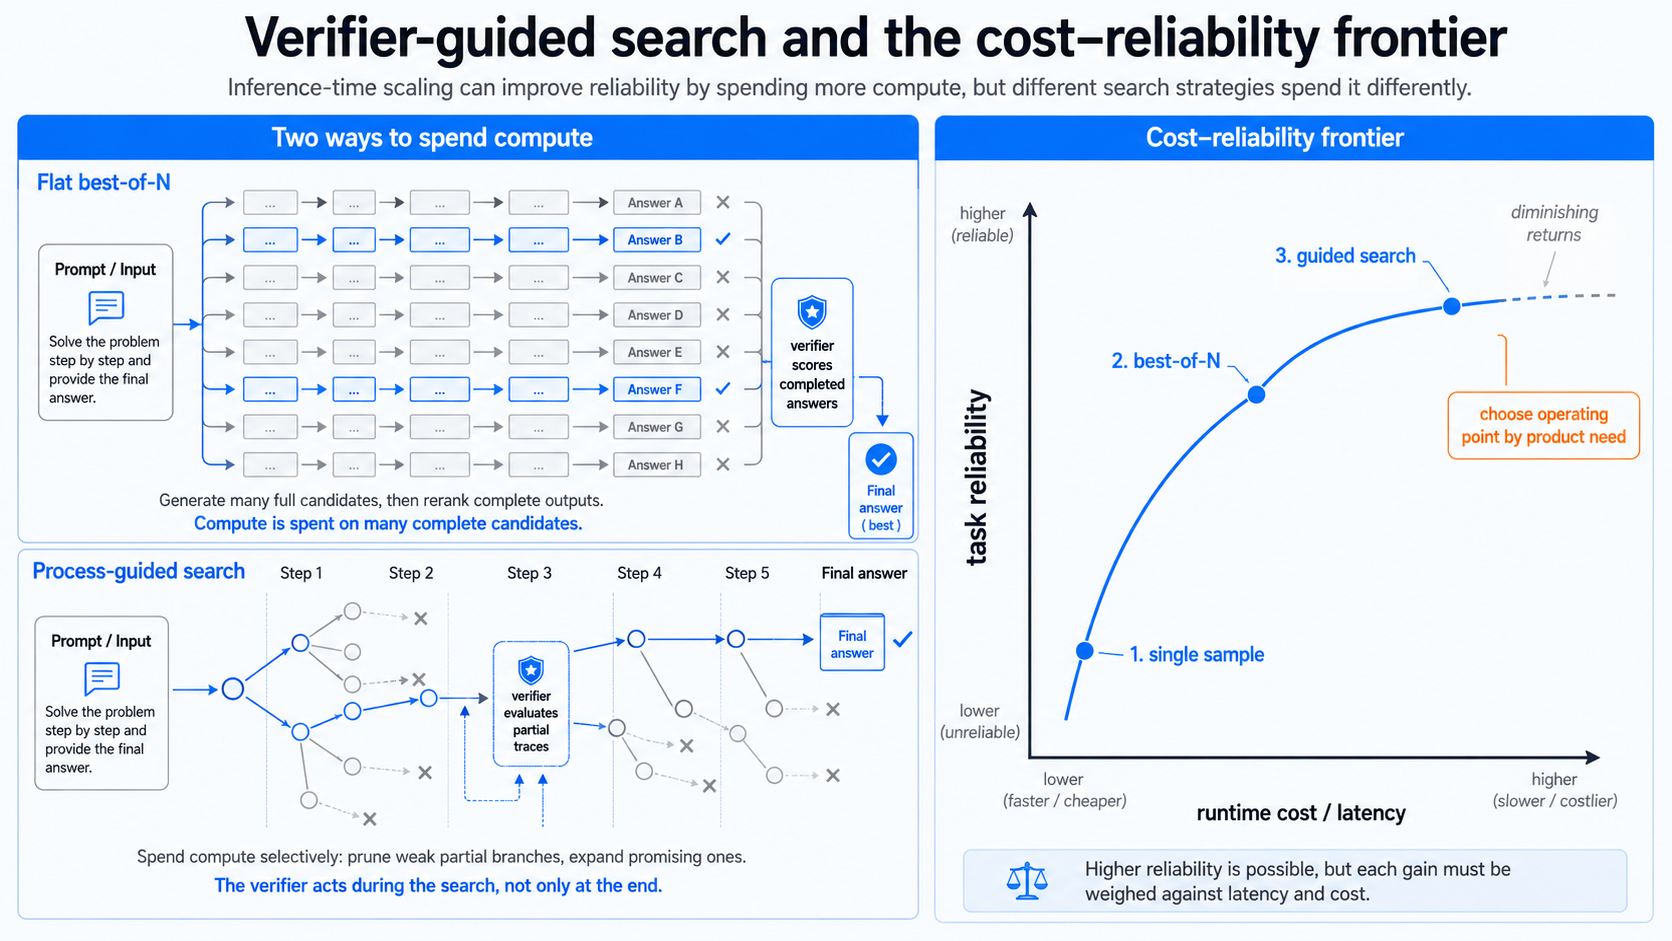
\includegraphics[width=0.95\textwidth]{figures/ch18/fig_verifier_search_frontier.png}
\caption{Verifier-guided search and the cost--reliability frontier. Flat best-of-$N$ spends compute on complete candidates; process-guided search spends compute adaptively on partial traces. Both must be judged by reliability gained per unit of latency and cost.}
\label{fig:ch18-verifier-search-frontier}
\end{figure}

\begin{quickrecap}
\textbf{Quick Recap.}
\begin{itemize}[nosep,leftmargin=1.5em]
  \item Search allocates compute over partial reasoning traces rather than complete answers only.
  \item The chapter's scope is model-internal search, not external tool-using agents.
  \item Search quality depends on the evaluator used to score partial states.
\end{itemize}
\textit{Next: all these methods must be paid for in latency, throughput, and dollars.}
\end{quickrecap}


%----------------------------------------------------------------------
\section{The Cost--Reliability Frontier}
\label{sec:ch18-cost-reliability}

Inference-time scaling is attractive because it can improve a fixed model. It is dangerous because it hides costs. Every extra sample consumes tokens. Every verifier call consumes compute. Every search branch increases latency. A deployed system must choose an operating point.

\subsection{A Simple Cost Model}

Let $N$ be the number of generated candidates. Let $C_{\text{gen}}$ be the cost of generating one candidate and $C_{\text{score}}$ the cost of scoring one candidate. A simple best-of-$N$ cost model is:

\begin{equation}
  C_{\text{total}} \approx N(C_{\text{gen}} + C_{\text{score}}).
  \label{eq:bestofn-cost}
\end{equation}

This ignores batching, cache reuse, different response lengths, and parallelism. Chapter~\ref{ch:serving-quantization-cost} will handle those serving details. For this chapter, the lesson is enough: best-of-$N$ usually buys reliability with roughly linear candidate cost, while accuracy often improves sublinearly.

Search has a similar budget, but the unit is not a complete candidate. It is a node expansion, a partial trace, or a verifier call. Adaptive search can be cheaper than fixed $N$ if it stops early on easy tasks and spends more on hard tasks.

\subsection{Latency Is Not the Same as Compute}

Generating 32 candidates in parallel may cost 32 times as much compute but not 32 times as much wall-clock latency if infrastructure allows batching. Generating them serially may be too slow for chat. A process verifier may reduce total tokens by pruning, but if the verifier is a large model called repeatedly, it can dominate latency.

This distinction is why Ch18 and Ch19 are separate. Ch18 asks which runtime algorithms improve reliability. Ch19 asks how serving systems make those algorithms affordable with batching, KV caches, quantization, scheduling, and throughput engineering.

\subsection{Operating Points}

Different products should choose different inference-time budgets:

\begin{itemize}[nosep]
  \item \textbf{Interactive chat}: low latency, small $N$, conservative decoding, maybe lightweight reranking.
  \item \textbf{Math homework solver}: moderate latency, self-consistency or verifier reranking.
  \item \textbf{Code generation batch job}: high latency tolerance, many samples, execution feedback, hidden tests.
  \item \textbf{Safety-critical advice}: do not rely on sampling alone; use external verification, abstention, and human review.
\end{itemize}

The same model can sit at different operating points depending on the task. This is why reporting a model's quality without decoding settings, sampling budget, and selection procedure is incomplete.

The running algebra problem should therefore have several reported scores, not one: greedy accuracy, pass@32, self-consistency accuracy, verifier-selected accuracy, average generated tokens, verifier calls, and latency. Those numbers describe the system's operating point.

\noindent\fbox{\parbox{\dimexpr\textwidth-2\fboxsep-2\fboxrule\relax}{%
\textbf{Pause and verify.}\quad A system can answer a request in three ways: single sample costs \$0.01 and succeeds 55\% of the time; best-of-8 costs \$0.08 and succeeds 76\% of the time; verifier-guided best-of-8 costs \$0.12 and succeeds 82\% of the time. Compute the added cost per percentage-point gain for each upgrade. Which operating point would you choose for interactive chat, and which for offline grading?
}}

\paragraph{The final rule.} Inference-time scaling converts compute into reliability only under two conditions: the model can generate useful alternatives, and the system has a selection signal that tracks the property you care about. If either condition fails, more compute mostly produces more expensive errors. The writing room shuts down when the writers cannot produce anything worth selecting, or when the editor cannot tell good writing from bad.

\begin{tcolorbox}[colback=orange!5, colframe=orange!60, title=\textbf{For Project~4: Report the Runtime Contract}]
When you build the agentic model system, report more than model name and prompt. Record temperature, top-$p$ or top-$k$, maximum tokens, number of samples, selector or verifier type, retry budget, latency, token cost, and final task success. If two systems use the same model but different runtime contracts, they are different systems.
\end{tcolorbox}


%----------------------------------------------------------------------
% End matter
%----------------------------------------------------------------------

\begin{takeaways}
\begin{enumerate}
  \item Autoregressive models produce next-token distributions; decoding decides how one candidate path is sampled.
  \item Greedy decoding is a fast baseline, not a measure of the model's full accessible behavior.
  \item Temperature, top-$k$, and top-$p$ control the diversity and tail risk of candidate generation.
  \item best-of-$N$ separates candidate generation from candidate selection; both stages can bottleneck performance.
  \item Self-consistency improves reasoning when sampled traces make partially independent errors.
  \item Verifier-guided inference uses outcome or process checks as runtime selection signals.
  \item Search over reasoning traces spends compute adaptively on partial paths, but only helps when the evaluator is reliable.
  \item The system-level question is the cost--latency--reliability frontier, not maximum accuracy at any cost.
\end{enumerate}
\end{takeaways}


\section*{Summary}

\paragraph{What this chapter established.} Ch18 turned a fixed post-trained model into a runtime system. The model supplies a token distribution. Decoding creates candidates. Sampling creates candidate pools. Voting, verifiers, and search choose among or expand those candidates. More inference compute can improve reliability, but only when the candidate pool contains useful alternatives and the selector can identify them.

\paragraph{The systems lesson.} Inference-time scaling is the first systems chapter because it introduces the central Part~IV habit: model quality is not a single number attached to weights. It depends on the runtime procedure around the weights. A deployment report that omits decoding settings, sampling budget, verifier type, and latency budget is missing the system.

\paragraph{One sentence.} \emph{Inference-time scaling is search over a fixed model's distribution under a cost budget.}

\paragraph{What comes next.} Chapter~\ref{ch:serving-quantization-cost} asks how to serve these runtime procedures efficiently: prefill and decode, KV-cache memory, batching, quantization, throughput, latency, and cost per useful task.

\section*{Key Equations}

\begin{center}
\small
\begin{tabularx}{\textwidth}{@{}p{3.5cm}p{5.2cm}X@{}}
\toprule
\textbf{Equation} & \textbf{Form} & \textbf{Why it matters} \\
\midrule
Next-token distribution & $p_\theta(x_t \mid x_{<t})$ & The model gives a distribution; decoding turns it into a sequence. \\
Temperature sampling & $p_T(x) = \exp(z_x/T) / \sum_{x'} \exp(z_{x'}/T)$ & Controls sharpness and diversity of sampled tokens. \\
pass@$k$ opportunity & $1-(1-p)^k$ & Estimates how often a candidate pool contains at least one success. \\
Selection decomposition & $\Pr(\text{success}) \approx a_N q$ & Separates candidate availability from selector quality. \\
best-of-$N$ cost & $C_{\text{total}} \approx N(C_{\text{gen}}+C_{\text{score}})$ & Shows why accuracy gains must be measured against compute and latency. \\
\bottomrule
\end{tabularx}
\normalsize
\end{center}

\section*{Key Checks}

\begin{center}
\small
\begin{tabularx}{\textwidth}{@{}p{3.7cm}p{5cm}X@{}}
\toprule
\textbf{Diagnostic} & \textbf{Question} & \textbf{Action} \\
\midrule
Decoding report & Are temperature, top-$p$, top-$k$, and max tokens specified? & Treat results without decoding settings as incomplete. \\
pass@$k$ curve & Does extra sampling keep improving, or does it saturate quickly? & Plot accuracy against $k$ under fixed decoding settings. \\
Selector audit & Does the selector choose correct candidates when they exist? & Evaluate candidate-pool oracle accuracy separately from selected accuracy. \\
Correlation check & Are samples meaningfully diverse or copies of the same mistake? & Cluster final answers and reasoning strategies, not only raw text. \\
Verifier independence & Is the runtime verifier checking the real target or a proxy? & Use held-out checks, hidden tests, or independent judges. \\
Cost frontier & How much accuracy does each extra sample or verifier call buy? & Report accuracy, latency, output tokens, verifier calls, and cost together. \\
\bottomrule
\end{tabularx}
\normalsize
\end{center}


\section*{Key Readings}

\begin{enumerate}[nosep]
  \item \textbf{Holtzman et al., 2020.} ``The Curious Case of Neural Text Degeneration''~\cite{holtzman2020curious}. The classic nucleus-sampling argument for truncating the unreliable tail.
  \item \textbf{Wang et al., 2023.} ``Self-Consistency Improves Chain of Thought Reasoning in Language Models''~\cite{wang2022selfconsistency}. The canonical multiple-reasoning-path voting method.
  \item \textbf{Cobbe et al., 2021.} ``Training Verifiers to Solve Math Word Problems''~\cite{cobbe2021gsm8k}. A key early example of verifier-guided mathematical reasoning.
  \item \textbf{Lightman et al., 2023.} ``Let's Verify Step by Step''~\cite{lightman2023verify}. Process supervision and step-level verification for reasoning.
  \item \textbf{Yao et al., 2023.} ``Tree of Thoughts''~\cite{yao2023tree}. A test-time search formulation over intermediate reasoning states.
  \item \textbf{Snell et al., 2024.} ``Scaling LLM Test-Time Compute Optimally Can be More Effective than Scaling Model Parameters''~\cite{snell2024scaling}. The compute-allocation framing that connects inference scaling back to model scaling.
  \item \textbf{DeepSeek-AI, 2025.} ``DeepSeek-R1''~\cite{deepseekai2025r1}. A public reasoning-model case where training-time and inference-time computation are tightly coupled.
\end{enumerate}

\flushbottom
